\documentclass{article}

\usepackage{minted}
\usepackage[most]{tcolorbox}
\usepackage{geometry}
\usepackage{enumitem}
\usepackage{hyperref}
\usepackage{hyperref}
\usepackage[parfill]{parskip}
\usepackage{wrapfig}
\usepackage{accsupp}

\geometry{margin=0.8in}
\definecolor{lightgreen}{rgb}{0.56, 0.93, 0.56}
\definecolor{moonstoneblue}{rgb}{0.45, 0.66, 0.76}
\definecolor{magenta}{rgb}{0.8,0.66,0.76}
\begin{document}
\BeginAccSupp{}
\begin{flushright}
Computational Biology ~\\
Tufts University Bio 35 ~\\
Fall 2021 ~\\ ~\\
\end{flushright}
\begin{center}{\textbf{\Large{Spotlight 13: Casey Overby Taylor}}}\end{center}

\textit{Please note that in general I have taken/adapted the words of our Spotlight subjects from their own websites to describe their work. I have done this in an effort to maintain accuracy in describing their research programs. Please do not copy paste text from their papers/websites in your assignments!}

\begin{wrapfigure}{L}{0.14\textwidth}
\begin{center}
 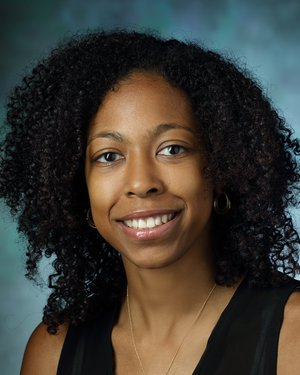
\includegraphics[width=0.13\textwidth]{images/overby-taylor.jpeg}
 \end{center}
\end{wrapfigure}
~\\ As part of our unit on precision medicine and human genomics, we are going to explore the work of Prof. Casey Overby Taylor. Dr. Overby Taylor's research draws from biomedical informatics and the related field of biomedical data science, to address the challenge of how to incorporate technology and digital approaches into clinical research and healthcare practices. She also draws from comparative effectiveness research approaches, including experience with conceptualizing and measuring implementation outcomes, to study the use of clinical decision support as a strategy to improve the adoption of clinically actionable guidance. Dr. Overby Taylor is Assistant Professor of Medicine and Biomedical Engineering at Johns Hopkins University. 
~\\

Please watch the following video:
\begin{enumerate}
\item \texttt{\href{https://www.youtube.com/watch?v=BKYGshY7Ggk}{https://www.youtube.com/watch?v=BKYGshY7Ggk}}
\end{enumerate}
And read the following article by Prof. Overby Taylor: 
\begin{enumerate}
\item \texttt{\href{https://www.nature.com/articles/gim2013128.pdf}{https://www.nature.com/articles/gim2013128.pdf}}
\end{enumerate}

\subsubsection*{Written Assignment} 
After reading about Casey Overby Taylor please write a reflection (max one page) on what you discovered. You might wish to address some of the following: 

\begin{enumerate}
\item What was most interesting to you in reviewing these resources?
\item What did you learn from these resources about personalized medicine and the role of genomic data in patient care?
\item What new questions do you have after reviewing these resources?
\item What do these resources tell you about the types of people that do computational biology, or their motivations?
\end{enumerate}
\EndAccSupp{}

\end{document}